\begin{qotdphybox}{PLAYING WITH THE BUBBLE}
\qotdtitle{101}{13}{01}
Two soap bubbles with surface tension coefficient $\sigma$ and radius $r$ are separated from each other by a planar thin soap film that has same surface tension coefficient by puncturing this membrane we can achieve a isothermal union of 2 bubbles, if the radius of newly formed bubble is $R$.
\begin{center}
    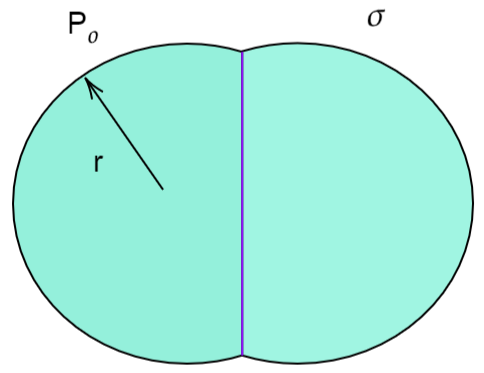
\includegraphics[width = .4\textwidth]{QoTD 101.png}
    \label{fig:qotd101}
\end{center}
\begin{qotdques}
\ques{4}
Then what is normal atmospheric pressure $P_o$ outside.
\ques{5}
What is interval in $r$ that $R$  changes over?
\end{qotdques}
\qotdcreator{v€çtørqûårk}
\end{qotdphybox}